\documentclass[a4paper,12pt]{article}
\usepackage[utf8]{inputenc}
\usepackage{amsmath}
\usepackage{bm} % to get bold epsilon
\usepackage{amssymb}
\usepackage{comment}
\usepackage{graphicx}
\usepackage[left=1.5cm, right=1.5cm, top=2cm, bottom=2cm]{geometry}
\title{\textbf{COM 5120 Communication Theory}}
\author{\textbf{Homework \#2 Solution}}
\date{Due at 23:59, December 20, 2022}
\begin{document}
    \maketitle
    % \textit{Note: }There are \textbf{6} problems with total 100 points within \textbf{3} pages, please write your answer with detail in the answer sheet.

    % {\bf No credit without detail.  No calculator. Closed books.}

    \begin{enumerate}
    %%%%%%%%%%%%%%%%%%%%%%%%%%%%%%
        \item 
            For the QAM signal constellation shown in Figure 1, determine the optimum decision boundaries for the detector, assuming that the SNR is sufficiently high that errors occur only between adjacent points.
            \begin{figure}[h]
            	\centering
            	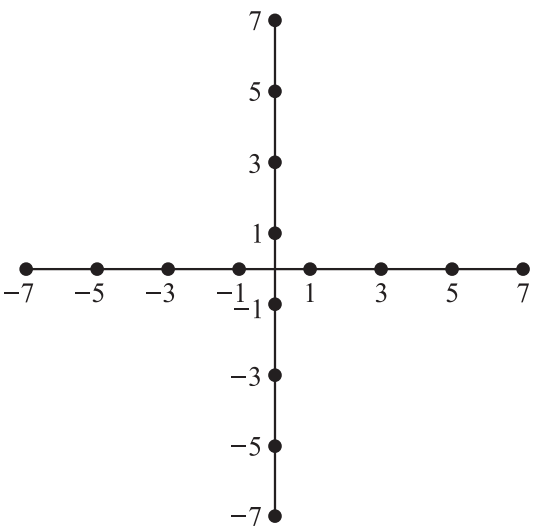
\includegraphics[scale=0.34]{HW2-1-1.png}
            	\caption{QAM signal constellation}
            % 	\label{fig}
            \end{figure} \\
            \textbf{Solution:} \\
            The optimum decision boundary of a point is determined by the perpendicular bisectors of each line segment connecting the point with its neighbors. The decision regions for this QAM constellation are depicted in Figure 2: \\ 
            \begin{figure}[h]
            	\centering
            	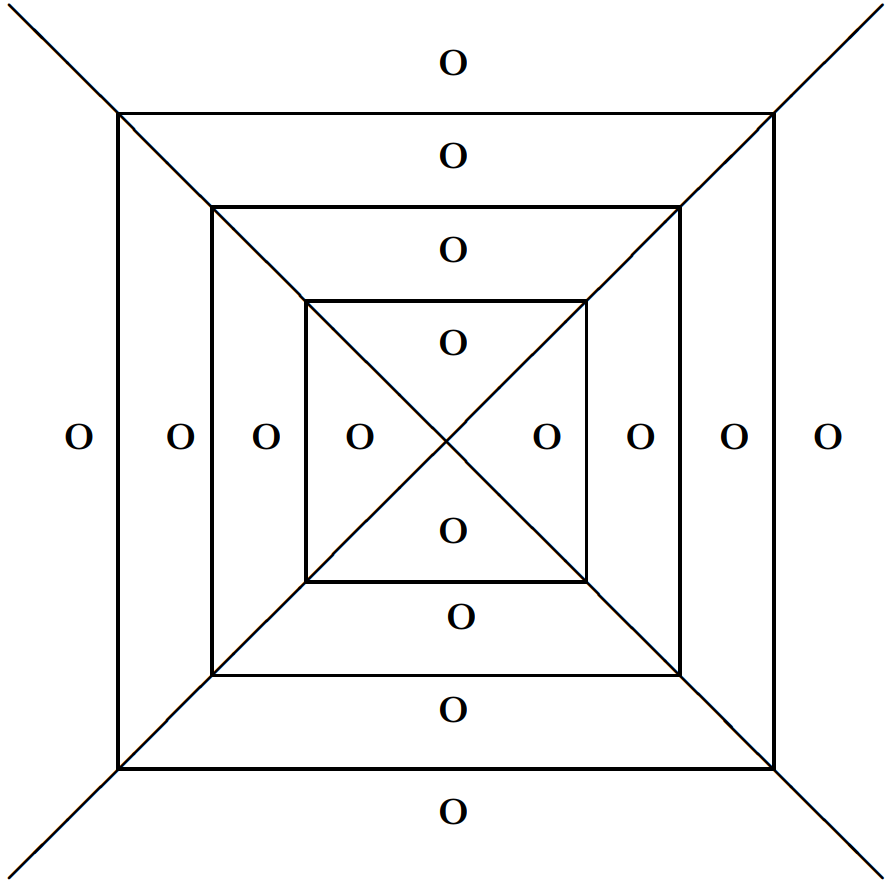
\includegraphics[scale=0.3]{HW2-1-2.png}
            	\caption{decision regions}
            % 	\label{fig}
            \end{figure}
            \begin{flushright}
                $\blacksquare$
            \end{flushright}
    %%%%%%%%%%%%%%%%%%%%%%%%%%%%%%
        \item
            Consider a digital communication system that transmits information via QAM over a voice-band telephone channel at a rate of $2400$ symbols/s. The additive noise is assumed to be white and Gaussian. \\
            (a) Determine the $\bm{\varepsilon_b} / N_0$ required to achieve an error probability of $10^{-5}$ at $4800$ bits/s. \\ 
            (b) Repeat part (a) for a rate of $9600$ bits/s. \\ 
            (c) Repeat part (a) for a rate of $19,200$ bits/s. \\ 
            (d) What conclusions do you reach from these results? \\  \\ 
            \textbf{Solution:} \\
            \textbf{(a)} The number of bits per symbol is $$k = \frac{4800}{R} = \frac{4800}{2400} = 2$$ Thus, a $4$-QAM constellation is used for transmission. The probability of error for an $M$-ary QAM system with $M = 2^k$, is $$P_M = 1 - \left( 1 - 2 \left( 1 - \frac{1}{\sqrt{M}} \right) Q \left[ \sqrt{\frac{3k\bm{\varepsilon_b}}{(M - 1) N_0}} \; \right] \right)^2$$ \\ 
            With $P_M = 10^{-5}$ and $k = 2$ we obtain $$Q \left[ \sqrt{\frac{2 \bm{\varepsilon_b}}{N_0}} \; \right] = 5 \cdot 10^{-6} \Rightarrow \frac{\bm{\varepsilon_b}}{N_0} = 9.7682$$ \\ 
            \textbf{(b)} If the bit rate of transmission is $9600$ bps, then $$k = \frac{9600}{R} = \frac{9600}{2400} = 4$$ In this case a $16$-QAM constellation is used and the probability of error is $$P_M = 1 - \left( 1 - 2 \left( 1 - \frac{1}{4} \right) Q \left[ \sqrt{\frac{3 \cdot 4 \cdot \bm{\varepsilon_b}}{15 \cdot N_0}} \; \right] \right)^2$$ Thus, $$Q \left[ \sqrt{\frac{3 \cdot \bm{\varepsilon_b}}{15 \cdot N_0}} \; \right] = \frac{1}{3} \cdot 10^{-5} \Rightarrow \frac{\bm{\varepsilon_b}}{N_0} = 25.3688$$ \\ 
            \textbf{(c)} If the bit rate of transmission is $19200$ bps, then $$k = \frac{19200}{R} = \frac{19200}{2400} = 8$$ In this case a $256$-QAM constellation is used and the probability of error is $$P_M = 1 - \left( 1 - 2 \left( 1 - \frac{1}{16} \right) Q \left[ \sqrt{\frac{3 \cdot 8 \cdot \bm{\varepsilon_b}}{255 \cdot N_0}} \; \right] \right)^2$$ With $P_M = 10^{-5}$ we obtain $$\frac{\bm{\varepsilon_b}}{N_0} = 659.8922$$ \\ 
            \newpage
            \textbf{(d)} The following table gives the SNR per bit and the corresponding number of bits per symbol for the constellations used in parts \textbf{(a)} - \textbf{(c)} 
            \begin{center}
                \begin{tabular}{ | c || c | c | c |} 
                 \hline
                 $k$ &  $2$ & $4$ & $8$ \\ 
                 \hline
                 SNR(db) & $9.89$ & $14.04$ & $28.19$ \\ 
                 \hline
                \end{tabular}
            \end{center}
            As it is observed there is an increase in transmitted power of approximately 3 dB per additional bit per symbol.
            \begin{flushright}
                $\blacksquare$
            \end{flushright}
    %%%%%%%%%%%%%%%%%%%%%%%%%%%%%%
        \item
            Let $X$ be a geometrically distributed random variable, i.e., $$P(X = k) = p(1-p)^{k - 1}, k = 1, 2, 3, ...$$
            (a) Find the entropy of $X$. \\ 
            (b) Given that $X > K$, where $K$ is a positive integer, what is the entropy of $X$? \\ \\ 
            \textbf{Solution:} \\
            \textbf{(a)} 
            \begin{align*}
                H(x) &= \ - \sum_{k = 1}^{\infty} p \left(1 - p\right)^{k - 1} \log_2 \left(p\left(1 - p\right)^{k - 1}\right) \\
                     &= \ -p \sum_{k = 1}^{\infty} \left(1 - p\right)^{k - 1} \log_2 p - p \sum_{k = 1}^{\infty} \left(1 - p\right)^{k - 1} \log_2 \left(1 - p\right)^{k - 1} \\ 
                     &= \ -p \log_2 p \sum_{k = 1}^{\infty} \left(1 - p\right)^{k - 1} - p \log_2 (1 - p) \sum_{k = 1}^{\infty} (k - 1)\left(1 - p\right)^{k - 1} \\
                     &= \ -p \log_2 p \ \frac{1}{1 - \left(1 - p\right)} - p \log_2 (1 - p) \ \frac{1 - p}{\left( 1 - \left(1 - p\right) \right)^2} \\ 
                     &= \ - \log_2 p - \frac{1 - p}{p} \log_2 (1 - p) \\ 
                \textbf{[Note]} \;\;\; & \sum_{k = 1}^{\infty} (k - 1)\left(1 - p\right)^{k - 1} = 0 + (1 - p) \cdot 1 + (1 - p)^2 \cdot 2 + \cdots = \sum_{k = 0}^{\infty} k \left(1 - p\right)^{k} \\ 
                                 & \text{Assume} \; \sum_{k = 0}^{\infty} k \left(1 - p\right)^{k} = S_n \;\;\; \text{and} \;\;
                                 \left\{ 
                                \begin{aligned}
                                    S_n &= 0 + (1 - p) \cdot 1 + (1 - p)^2 \cdot 2 + \cdots \\
                                    (1 - p)S_n &= 0 + 0 + (1 - p)^2 \cdot 1 + \cdots \\ 
                                \end{aligned}
                                \right. \\ 
                                 % & S_n = 0 + (1 - p) \cdot 1 + (1 - p)^2 \cdot 2 + \cdots \\ 
                                 % & (1 - p)S_n = 0 + 0 + (1 - p)^2 \cdot 1 + \cdots \\ 
                                 & \Rightarrow S_n - (1 - p)S_n = 0 + (1 - p) + (1 - p)^2 + \cdots \\ 
                                 & \Rightarrow \left[ 1 - (1 - p) \right] S_n = \sum_{k = 1}^{\infty} \left(1 - p\right)^{k} = \frac{1 - p}{1 - (1 - p)} \\
                                 & \Rightarrow S_n = \frac{1 - p}{\left[ 1 - (1 - p) \right]^2}
            \end{align*} 
            \textbf{(b)} 
            Clearly $P(X = k | X > K) = 0$ for $k \leq K$. If $k > K$, then $$P(X = k | X > K) = \frac{P(X = k, X > K)}{P(X > K)} = \frac{p(1 - p)^{k - 1}}{P(X > K)}$$ But, 
            \begin{align*}
                P(X > K) &= \ \sum_{k = K + 1}^{\infty} p \left(1 - p\right)^{k - 1} \\
                         &= \ p \left( \sum_{k = 1}^{\infty} \left(1 - p\right)^{k - 1} - \sum_{k = 1}^{K} \left(1 - p\right)^{k - 1} \right) \\
                         &= \ p \left( \frac{1}{1 - (1 - p)} - \frac{1 - (1 - p)^K}{1 - (1 - p)} \right) \\ 
                         &= \ (1 - p)^K \\ 
            \end{align*}
            so that $$P(X = k | X > K) = \frac{p(1 - p)^{k - 1}}{(1 - p)^K}$$
            If we let $k = K + l$ with $l = 1, 2, 3, ...$ then $$P(X = k | X > K) = \frac{p(1 - p)^K (1 - p)^{l - 1}}{1 - p)^K} = (1 - p)^{l - 1}$$
            that is $P(X = k | X > K)$ is the geometrically distributed. Hence, using the results of the first part we obtain 
            \begin{align*}
                H(X | X > K) &= \ - \sum_{l = 1}^{\infty} p(1 - p)^{l - 1} \log_2 \left( p(1 - p)^{l - 1} \right) \\
                             &= \ - \log_2 p - \frac{1 - p}{p} \log_2 \left(1 - p\right) \\
            \end{align*}
            \begin{flushright}
                $\blacksquare$
            \end{flushright}
            % \newpage
    %%%%%%%%%%%%%%%%%%%%%%%%%%%%%    
        \item 
            A DMS has an alphabet of eight letters $\; x_i, \ i = 1, 2,..., 8,$ with probabilities $\ 0.25$, $0.20$, $0.15$, $0.12$, $0.10$, $0.08$, $0.05$, and $0.05$. \\
            (a) Use the Huffman encoding procedure to determine a binary code for the source output. \\ 
            (b) Determine the average number $\Bar{R}$ of binary digits per source letter. \\ 
            (c) Determine the entropy of the source and compare it with $\Bar{R}$. \\ \\ 
            \textbf{Solution:} \\
            \textbf{(a)} 
            Figure 3 depicts the design of a ternary Huffman code (we follow the convention that the lower-probability branch is assigned a 1):
            \begin{figure}[h]
                \centering
                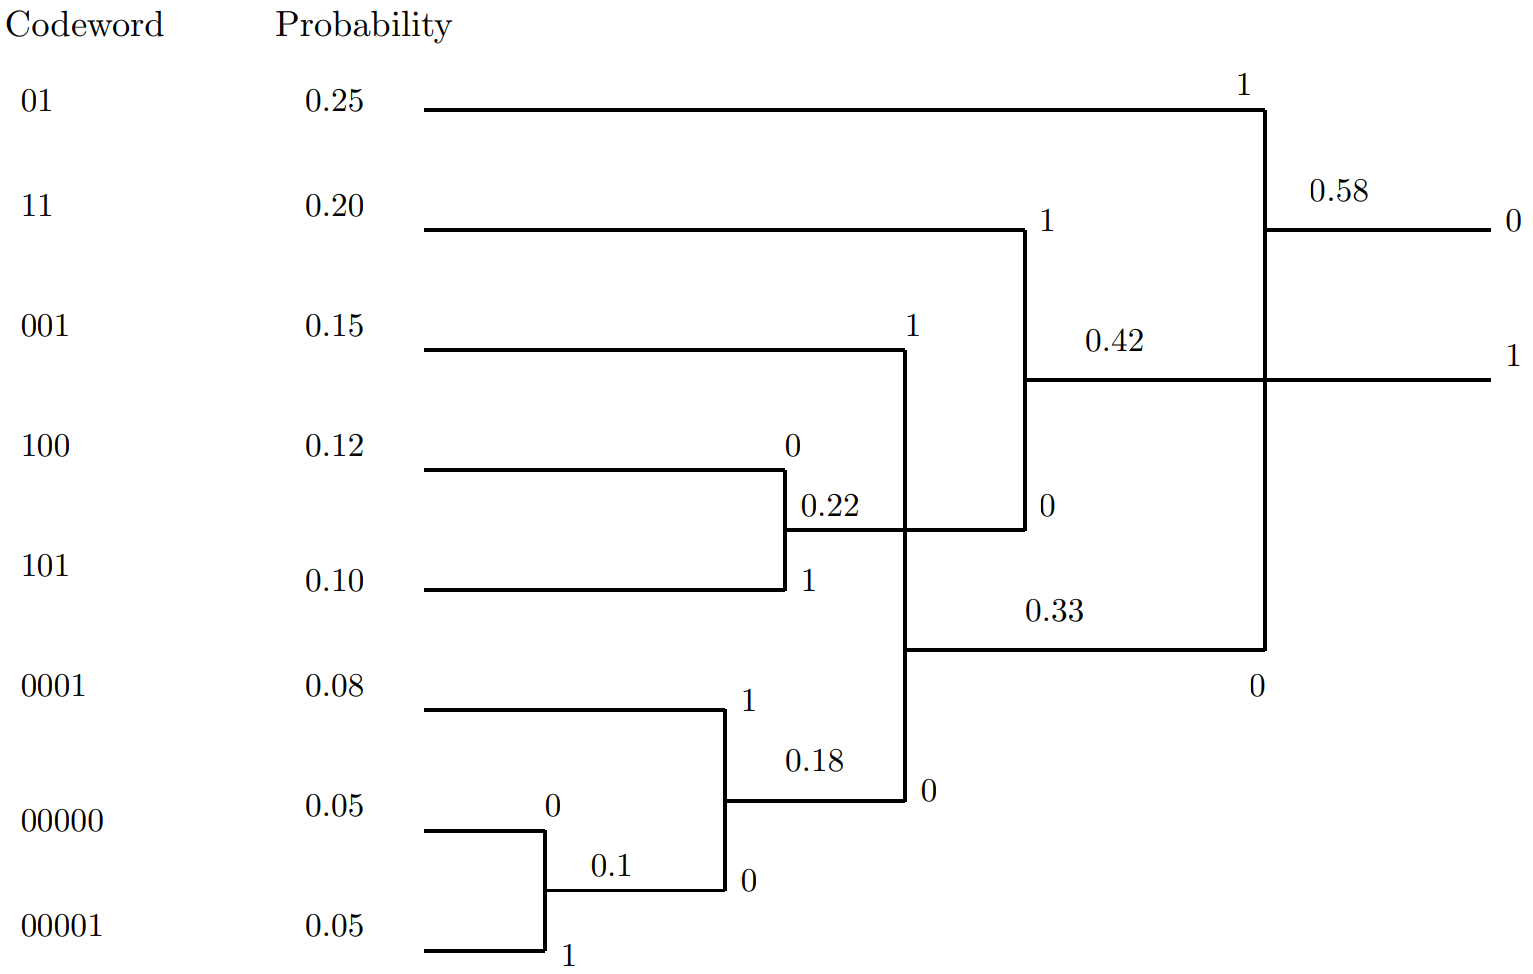
\includegraphics[scale=0.4]{HW2-4-1.png}
                \caption{ternary Huffman code}
                % \label{fig:my_label}
            \end{figure} \\ 
            \textbf{(b)} 
            The average number of binary digits per source letter is: $$\Bar{R} = \sum_{i}^{}P(x_{i})n_{i} = 2 \times 0.45 + 3 \times 0.37 + 4 \times 0.08 + 5 \times 0.1 = 2.83 \;\; \text{bits/letter}$$
            \textbf{(c)} 
            The entropy of the source is: $$H(X) = - \sum_{i}^{}P(x_{i}) \log P(x_{i}) = 2.80 \;\; \text{bits/letter}$$
            As it is expected the entropy of the source is less than the average length of each codeword.
            \begin{flushright}
                $\blacksquare$
            \end{flushright}
    %%%%%%%%%%%%%%%%%%%%%%%%%%%%%%%%%%%%%%%%%%%%%%    
        \item 
            A discrete memoryless source has an alphabet of size 7, $\mathcal{X} = \{ x_1, \ x_2, \ x_3, \ x_4, \ x_5, \ x_6, \ x_7 \}$, with corresponding probabilities $\{ 0.02, \ 0.11, \ 0.07, \ 0.21, \ 0.15, \ 0.19, \ 0.25 \}$. \\
            (a) Determine the entropy of this source. \\ 
            (b) Design a Huffman code for this source, and find the average codeword length of the Huffman code. \\ 
            (c) A new source $\mathcal{Y} = \{ y_1, \ y_2, \ y_3 \}$ is obtained by grouping the outputs of the source $\mathcal{X}$ as 
            % $ y_1 = \{ x1, \ x2, \ x5 \}, \; y_2 = \{ x3, \ x7 \}, \; y_3 = \{ x4, \ x6 \}$ 
            $$ 
            \begin{aligned}
                & y_1 = \{ x1, \ x2, \ x5 \} \\
                & y_2 = \{ x3, \ x7 \} \\ 
                & y_3 = \{ x4, \ x6 \} \\
            \end{aligned}
            $$ \\
            Determine the entropy of $\mathcal{Y}$. \\
            (d) Which source is more predictable, $\mathcal{X}$ or $\mathcal{Y}$ ? Why? \\ \\
            \textbf{Solution:} \\
            \textbf{(a)} 
            The entropy is $$H(X) = - \sum_{i = 1}^{7} p_i \log_2 p_i \thickapprox 2.5703$$
            \textbf{(b)} 
            The Huffman tree is shown below in Figure 4
            \begin{figure}[h]
                \centering
                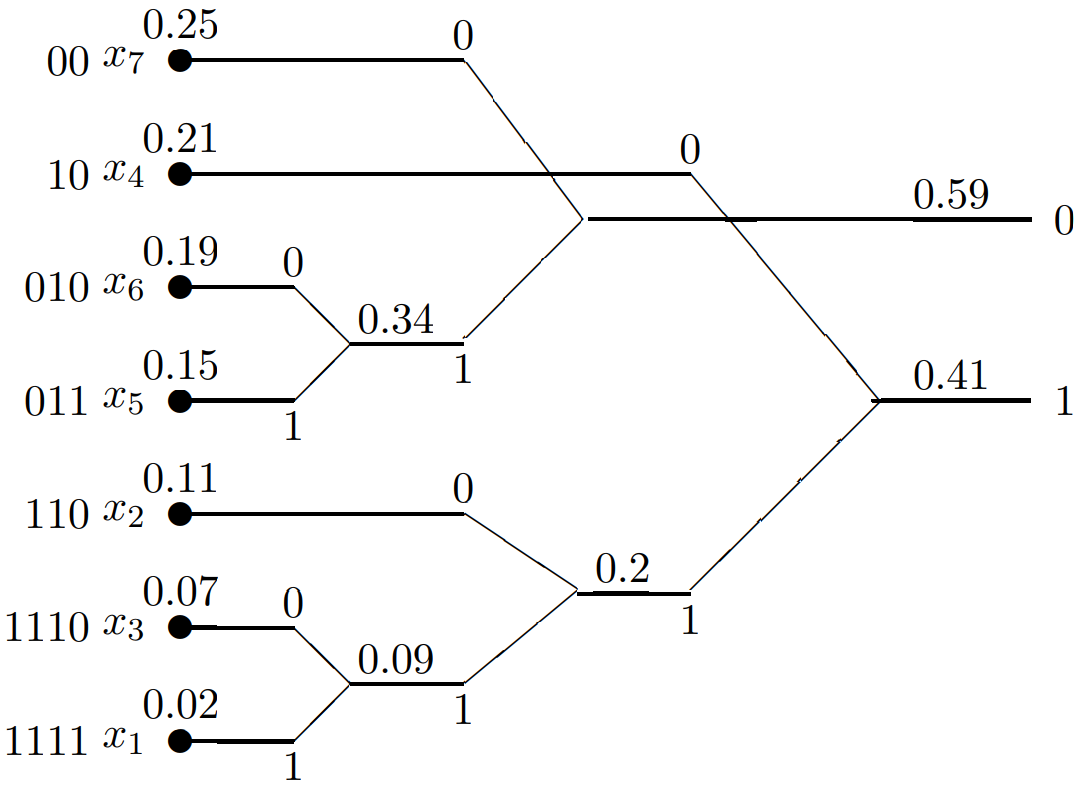
\includegraphics[scale=0.4]{HW2-5-1.png}
                \caption{Huffman tree}
                % \label{fig:my_label}
            \end{figure} \\ 
            and $$\Bar{R} = \sum_{i}^{}P(x_{i})n_{i} = 2 \times (0.25 + 0.21) + 3 \times (0.19 + 0.15 + 0.11) + 4 \times (0.07 + 0.02) = 2.63$$
            \textbf{(c)} 
            We have
            $$ 
            \begin{aligned}
                & P(y_1) = 0.02 + 0.11 + 0.15 = 0.28 \\
                & P(y_2) = 0.07 + 0.025 = 0.32 \\ 
                & P(y_3) = 0.21 + 0.19 = 0.4 \\
            \end{aligned}
            $$
            Therefore, $$H(Y) = \sum_{j = 1}^{3} P(Y_j) \log_2 P(Y_j) \thickapprox 1.569$$
            \textbf{(d)}
            $\mathcal{Y}$ is more predictable because its entropy is lower.
            \begin{flushright}
                $\blacksquare$
            \end{flushright}
    %%%%%%%%%%%%%%%%%%%%%%%%%%%%%%
        \item 
            A memoryless source has the alphabet $A = \{-5, \ -3, \ -1, \ 0, \ 1, \ 3, \ 5 \}$, with corresponding probabilities $\{ 0.05, \ 0.1, \ 0.1, \ 0.15, \ 0.05, \ 0.25, \ 0.3 \}$. \\ 
            (a) Find the entropy of the source. \\ 
            (b) Assuming that the source is quantized according to the quantization rule
            $$\left\{ 
            \begin{aligned}
                & q(-5) = q(-3) = -4 \\
                & q(-1) = q(0) = q(1) = 0 \\ 
                & q(3) = q(5) = 4 \\
            \end{aligned}
            \right.
            $$ 
            find the entropy of the quantized source. \\ \\
            \textbf{Solution:} \\
            \textbf{(a)} 
            \begin{align*}
                H(X) = -( & 0.05 \log_2 0.05 + 0.1 \log_2 0.1 + 0.1 \log_2 0.1 + 0.15 \log_2 0.15 \\ & + 0.05 \log_2 0.05 + 0.25 \log_2 0.25 + 0.3 \log_2 0.3) = 2.5282
            \end{align*}
            % $$H(X) = -(0.05 \ \log_2 0.05 \ + \ 0.1 \ \log_20.1 \ + \ 0.1 \ \log_2 \ 0.1 \ + \ 0.15 \ \log_2 \ 0.15 \ + \ 0.05 \ \log_2 \ 0.05 \ + \ 0.25 \ \log_2 \ 0.25  \ + \ 0.3 \ \log_2 \ 0.3) = 2.5282$$
            \textbf{(b)} 
            After quantization, the new alphabet is $B = \{ -4, 0, 4 \}$ and the corresponding symbol probabilities are given by
            $$ 
            \begin{aligned}
                & P(-4) = P(-5) + P(-3) = 0.05 + 0.1 = 0.15 \\
                & P(0) = P(-1) + P(0) + P(1) = 0.1 + 0.15 + 0.05 = 0.3 \\ 
                & P(4) = P(3) + P(5) = 0.25 + 0.3 = 0.55 \\
            \end{aligned}
            $$
            Hence, $H(Q(X)) = 1.4060$. As it is observed quantization decreases the entropy of the source.
            \begin{flushright}
                $\blacksquare$
            \end{flushright}
            % \newpage
    %%%%%%%%%%%%%%%%%%%%%%%%%%%%%%%%%%%%%%%%%%%%%%
    \end{enumerate}
    \rule{\textwidth}{0.4pt}
\end{document}


